\chapter{Assignment 3}
The first problem is solvable with yices. This can be expressed as an SMT problem with linear integer equations.  In these linear equations $S_i$ refers to the start of job $i$ with length $i$.

To express this problem in an SMT problem, 2 general predicate are defined. The first predicate makes sure that job $a$ is after job $b$. This can be expressed as follows: $S_{a} \ge S_{b} + b$. This predicate is called $precedence(a, b)$. The second predicate is that 2 jobs, namely $a$ and $b$, do not overlap. This is called $dont\_overlap(a, b)$ and can be expressed as follows:
\begin{align*}
&\neg (S_a \ge S_b \land S_a < S_b + b) \\
\land &\neg (S_a + a > S_b \land S_a + a \le S_b + b) \\
\land &\neg (S_b \ge S_a \land S_b < S_a + a) \\
\land &\neg (S_b + b > S_a \land S_b + b \le S_a + a) 
\end{align*}

Then the resulting problem becomes quite easy. We assume there is a list $P$ with all the precedences. Also a list $C$ with all the jobs that can not run concurrently.

\begin{align*}
\forall_{<a,b> \in P}& \; precedence(a, b) \\
\forall_{<a,b> \in C}& \; dont\_overlap(a, b) \\
\forall_{1 \le i \le 12}& \; S_i \ge 0
\end{align*}

The total resulting span of the jobs is 36. The resulting plan is plotted in \ref{fig:assignments3}.

\begin{figure}
	\centering
	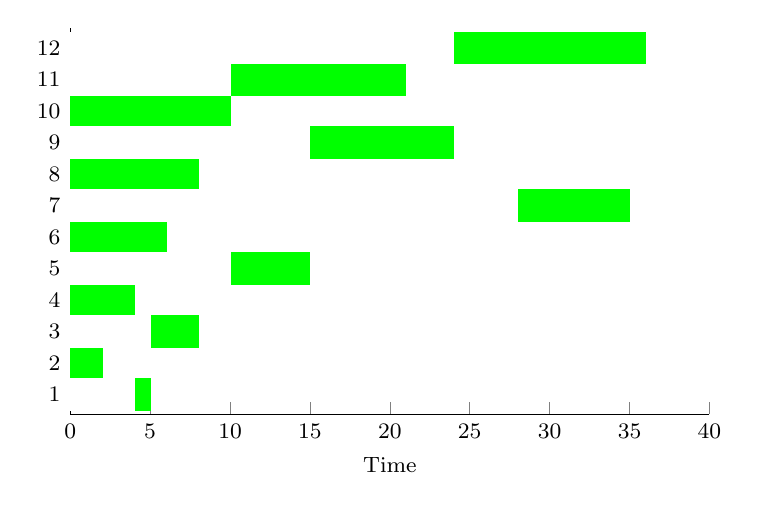
\begin{tikzpicture}
	\begin{axis}[
	xbar stacked,
	legend style={
		legend columns=4,
		at={(xticklabel cs:0.5)},
		anchor=north,
		draw=none
	},
	ytick=data,
	axis y line*=none,
	axis x line*=bottom,
	tick label style={font=\footnotesize},
	legend style={font=\footnotesize},
	label style={font=\footnotesize},
	xtick={0,5,10,15,20,25,30,35,40},
	width=.8\textwidth,
	bar width=4mm,
	xlabel={Time},
	yticklabels={1, 2, 3, 4, 5, 6, 7, 8, 9, 10, 11, 12},
	xmin=0,
	xmax=40,
	area legend,
	y=4mm,
	enlarge y limits={abs=0.625},
	]
	
	\addplot[white,fill=white] coordinates
	% starts
	{(4,1) (0,2) (5,3) (0,4) (10,5) (0,6) (28,7) (0,8) (15,9) (0,10) (10,11) (24,12)};
	
	\addplot[green,fill=green] coordinates
	% ends
	{(1,1) (2,2) (3,3) (4,4) (5,5) (6,6) (7,7) (8,8) (9,9) (10,10) (11,11) (12,12)};
	
	%\legend{Transfer,Database,Transfer,Rendering}
	\end{axis}
	\end{tikzpicture}
	\caption{Planning results}
	\label{fig:assignments3}
\end{figure}
